Modern experimental neuroscience research relies on training animals in tasks that isolate or exacerbate demands for specific cognitive variables of interest \citep{Gomez-Marin2016}. Given the non-verbal nature of most subjects, stable performance in such paradigms is often achieved through the successive reinforcement of simpler behaviors, a process known as “shaping” \citep{Jones1939}. These reinforcers may take several forms. Nevertheless, for both historical and practical reasons, liquid rewards have become a staple in most widely studied animal models \citep{Guo2014}. 

Due to their simplicity and compactness, gravity-based passive systems, most commonly implemented using valves, are widely adopted by the neuroscience community. With this approach, the volume of the delivered fluid is determined by the duration a valve remains open. Despite their convenience, gravity-based systems routinely face operational issues. First, due to changes in the fluid resistance (e.g.: biofilm growth in tubing), calibration values tend to drift across days, requiring frequent maintenance and re-calibration. Second, the relationship between reward amount and valve opening time is often non-linear, especially for small volumes, requiring calibration over several reward sizes. Finally, since the fluid flow rate is constant under a given value of hydraulic pressure, it is challenging to decouple delivered liquid volume from the total delivery time.

Alternative active systems, such as syringe pumps, have the potential to solve all the aforementioned problems. Unfortunately, currently available commercial systems are prohibitively expensive, often lack a flexible control system to fully satisfy the experimental needs of the users, and are difficult to implement at scale.

Here, we present and characterize an open-source syringe pump system (\cref{fig:PumpDrawing}) with scalable neuroscience experiments in mind. We provide detailed instructions and a parts-list that allow the system to be fully assembled using widely available off-the-shelf and custom 3D printed parts. 
In addition to mechanical designs, we also developed a flexible control system that affords a large range of customizability over the system's function. This control is implemented in a custom-designed printed circuit board (PCB) that implements the Harp protocol.

Additionally, the provided designs allow users to control the pump in a variety of ways. From triggering pre-defined protocols with a single square pulse to fully specify the behavior of the pump using the Harp Protocol. The latter interface, affords communication with Bonsai \citep{Lopes2015}, which in turn integrates the device in an ever increasing ecosystem of software for experimental behavior control and acquisition.

Similarly to other open-source systems \citep{Wijnen2014, Amarante2019}, we characterized the error associated with the delivery of large volumes. Additionally, since rodent experiments often rely on the delivery of microlitre range rewards we also designed a simple assay, leveraging computer vision, to characterize the performance of the pump in single-bolus events.

To validate the usefulness of the system, we varied the amount of reward delivered and show that this manipulation can quickly and reversibly alter rat's choice behavior. Finally, we highlight the high compatibility of the described syringe pump with electrophysiology recordings, and demonstrate no detectable electric artifact was observed.


\begin{figure*}
	\centering
	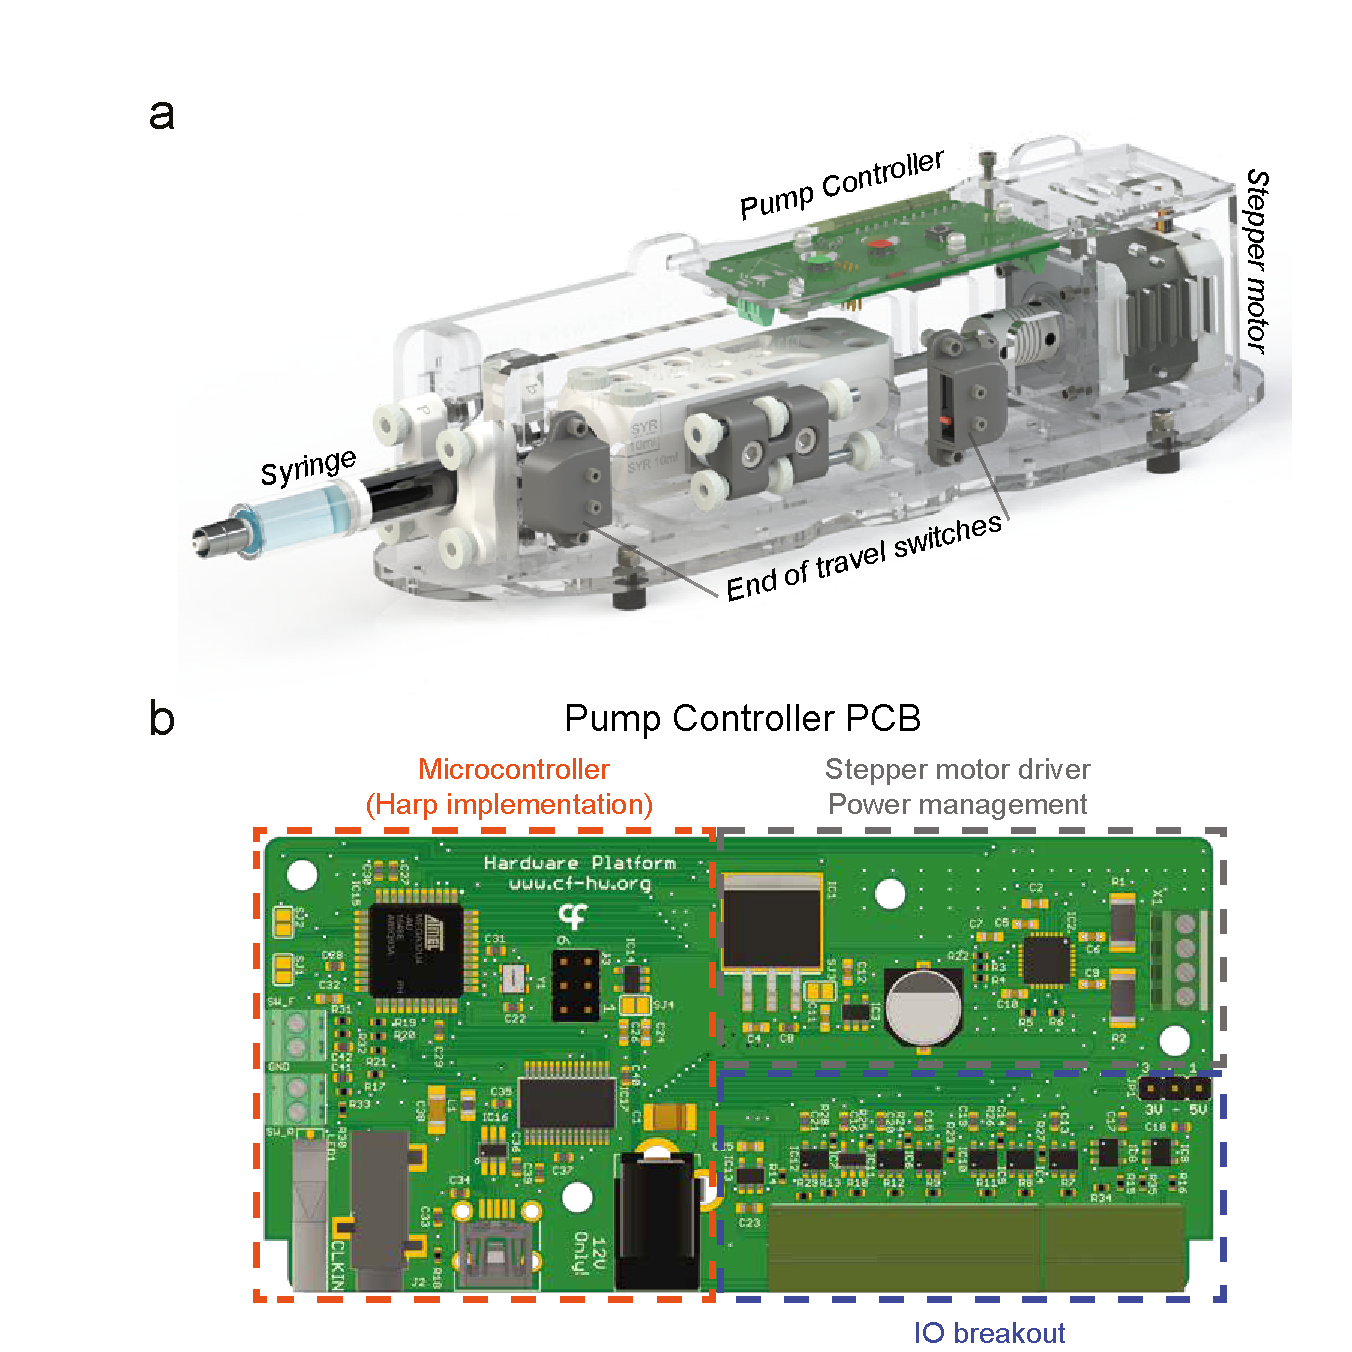
\includegraphics[width=1.0\linewidth]{Figures/Artboard 1.pdf}
	\caption{\textbf{Syringe pump system.}\\
		(\textbf{a}) 3D model of the fully assembled syringe pump system. Controller PCB, syringe, switches, and stepper motor are highlighted.  (\textbf{b}) Diagram of Controller PCB. The three main sections of the board are highlighted: Microcontroller, which implements the Harp protocol. Motor driver and power, which provide the low-level logic to drive the stepper motor, and the I/O breakout, that affords users with input and output lines which can be used to control and monitor the function of the system, respectively. See \hyperref[s:methods]{Methods} for further details}
	\label{fig:PumpDrawing}
\end{figure*}
